% 1977 年江苏连云港市初试卷附加题（第 9 题）：双曲线 x²-y²=1 上一点 A，
% A 点处法线交坐标轴于 B（Y 轴）、C（X 轴），B、A、C 三点共线（按源卷第 3 页「附加题」布局，取样例点示意）
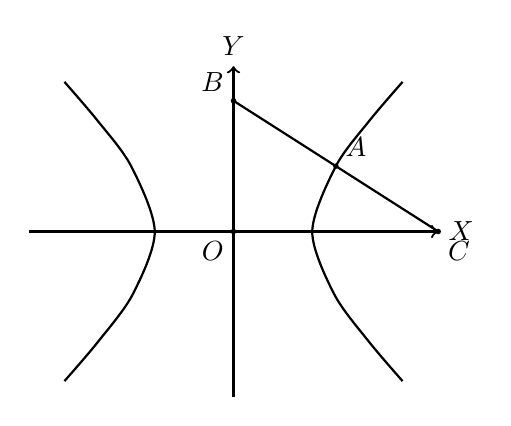
\begin{tikzpicture}[scale=1]
  \draw[thick,->] (-2.6,0) -- (2.6,0) node[right] {$X$};
  \draw[thick,->] (0,-2.1) -- (0,2.1) node[above] {$Y$};
  \draw[thick] plot[smooth] coordinates {(2.147,-1.9) (1.720,-1.4) (1.281,-0.8) (1,0) (1.3,0.83) (1.720,1.4) (2.147,1.9)};
  \draw[thick] plot[smooth] coordinates {(-2.147,-1.9) (-1.720,-1.4) (-1.281,-0.8) (-1,0) (-1.3,0.83) (-1.720,1.4) (-2.147,1.9)};
  \coordinate (O) at (0,0);
  \coordinate (B) at (0,1.66);
  \coordinate (A) at (1.3,0.83);
  \coordinate (C) at (2.6,0);
  \draw[thick] (B) -- (C);
  \fill (O) circle (1pt) node[below left] {$O$};
  \fill (B) circle (1pt) node[above left] {$B$};
  \fill (A) circle (1pt) node[above right] {$A$};
  \fill (C) circle (1pt) node[below right] {$C$};
\end{tikzpicture}
